\documentclass[PMO,authoryear,toc,daft]{lsstdoc}
% lsstdoc documentation: https://lsst-texmf.lsst.io/lsstdoc.html
\input{meta}

% Package imports go here.

% Local commands go here.

%If you want glossaries
%\input{aglossary.tex}
%\makeglossaries

\title{Enable Two-factor Authentication For OpenVPN}

% Optional subtitle
% \setDocSubtitle{A subtitle}

\author{%
Hernán Stockebrand
}

\setDocRef{ITTN-053}
\setDocUpstreamLocation{\url{https://github.com/lsst-it/ittn-053}}

\date{\vcsDate}

% Optional: name of the document's curator
% \setDocCurator{The Curator of this Document}

\setDocAbstract{%
Activate two-factor authentication on VPN connection for Rubin Observatory Users.
}

% Change history defined here.
% Order: oldest first.
% Fields: VERSION, DATE, DESCRIPTION, OWNER NAME.
% See LPM-51 for version number policy.
\setDocChangeRecord{%
  \addtohist{1}{YYYY-MM-DD}{Unreleased.}{Hernán Stockebrand}
}


\begin{document}

% Create the title page.
\maketitle
% Frequently for a technote we do not want a title page  uncomment this to remove the title page and changelog.
% use \mkshorttitle to remove the extra pages

% ADD CONTENT HERE
% You can also use the \input command to include several content files.
\section{Introduction}

The MFA is a way of computer access control to secure data and applications,  in a way that a user must prove with two or more ways his identity. 
It can be with a password, a time-based one-time password\textbf{ (TOTP),} a digital certificate, or bio metrics.

Two-factor authentication \textbf{(2FA)} is a method that combines just two of the previously mentioned components. Multi-Factor authentication \textbf{(MFA) }combines more than two components.

\textbf{MFA} increases security because if just one of the credentials is compromised, the unauthorized user will not be able to know the MFA authentication requirement, and the access will be denied.


\subsection{How Multi-Factor Authentication Works?
}
Because MFA needs at least two credentials at login to verify the identity before granting access. Each additional layer of authentication to the login increases security.

MFA requires the combination of the following:


\begin{itemize}
\item \textbf{Knowledge}- \textbf{Something you Know}: Password, pin, or answer to security questions
\item \textbf{Possession}-\textbf{Something you Have}: Smart Card, Mobile token, hardware token.
\item \textbf{Inherence} -\textbf{Something you Are}: Bio-metrics, voice recognition, fingerprint.
\end{itemize}

\newpage
\section{Requirements}
 
The IT requirements are the following:

\begin{itemize}
\item Add and extra layer of security to the VPN connection.
\item This can be an OTP or a "push" notification to an smartphone
\item Compatibility with our systems
\item Minor changes on our infrastructure for deployment
\item Achieve regulatory compliance
\end{itemize}

\newpage

\section{FreeIPA + OTP}

\begin{figure}
  \centering
  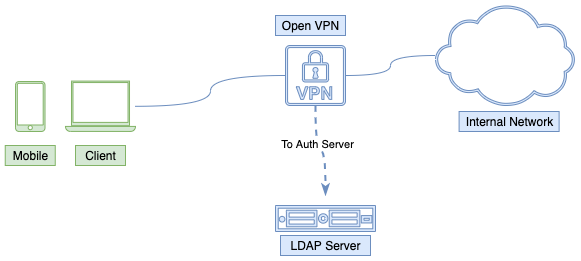
\includegraphics[width=160mm]{images/Pfsense - FreeIPA.drawio.png}
  \caption{OpenVPN + FreeIPA Authentication Server}
  \label{fig:label}
\end{figure}


\href{https://www.freeipa.org}{FreeIPA}   is a free and opensource Identity Managment System, aims to provide a centrally managed Identity, Policy and Audit (IPA)

FreeIPA native supports OTP authentication, and it can be enabled with just a few click inside a user profile, then a QR code is generated and is can be scan with an Smartphone with the app 
 \href{https://freeotp.github.io/ }{FreeOTP}.

\begin{figure}
    \centering
    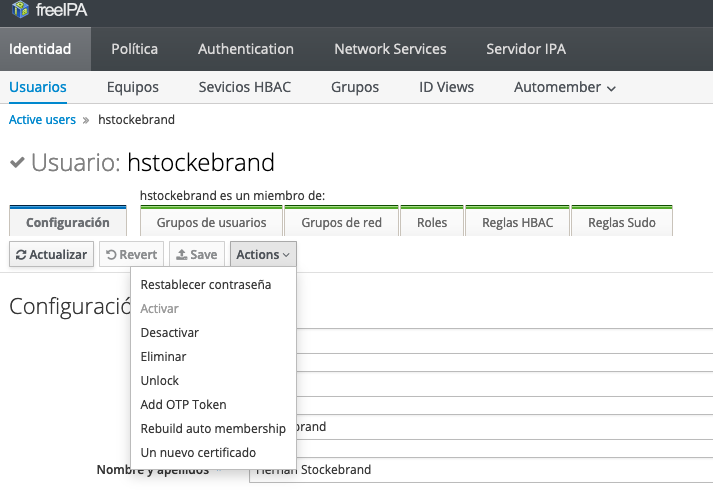
\includegraphics[width=140mm]{images/enable_OTP_IPA.png}
    \caption{Enable OTP on IPA}
    \label{fig:label}
\end{figure}

\newpage

\begin{figure}
    \centering
    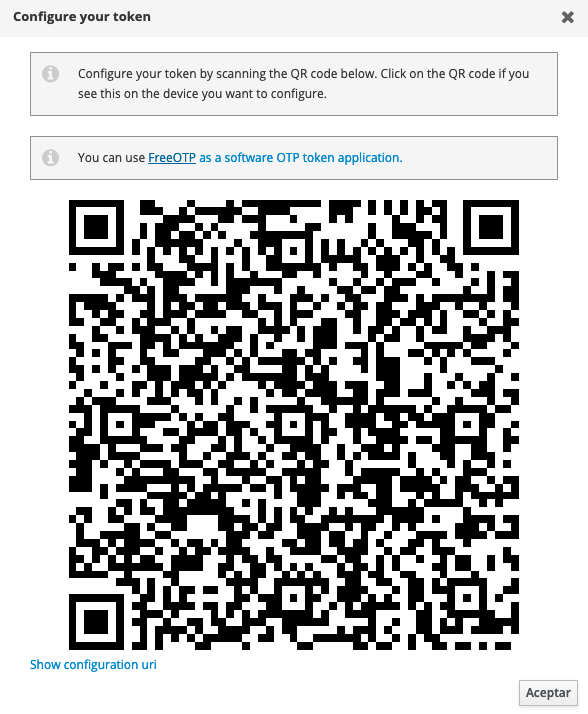
\includegraphics[width=60mm]{images/qr_code.png}
    \caption{QR Code to be Scan with the suggested app}
    \label{fig:label}
\end{figure}

No other change on any other service is needed, because this is transparent to the VPN service.

\newpage
\subsection{Test}

In our test, when connecting with the VPN client, on this case OpenVPN Connect, there is no aditional field or box requesting the aditional OTP code, so the user password and OTP code must be write togheter on the password field, as the example shows on the next image

\begin{figure}
    \centering
    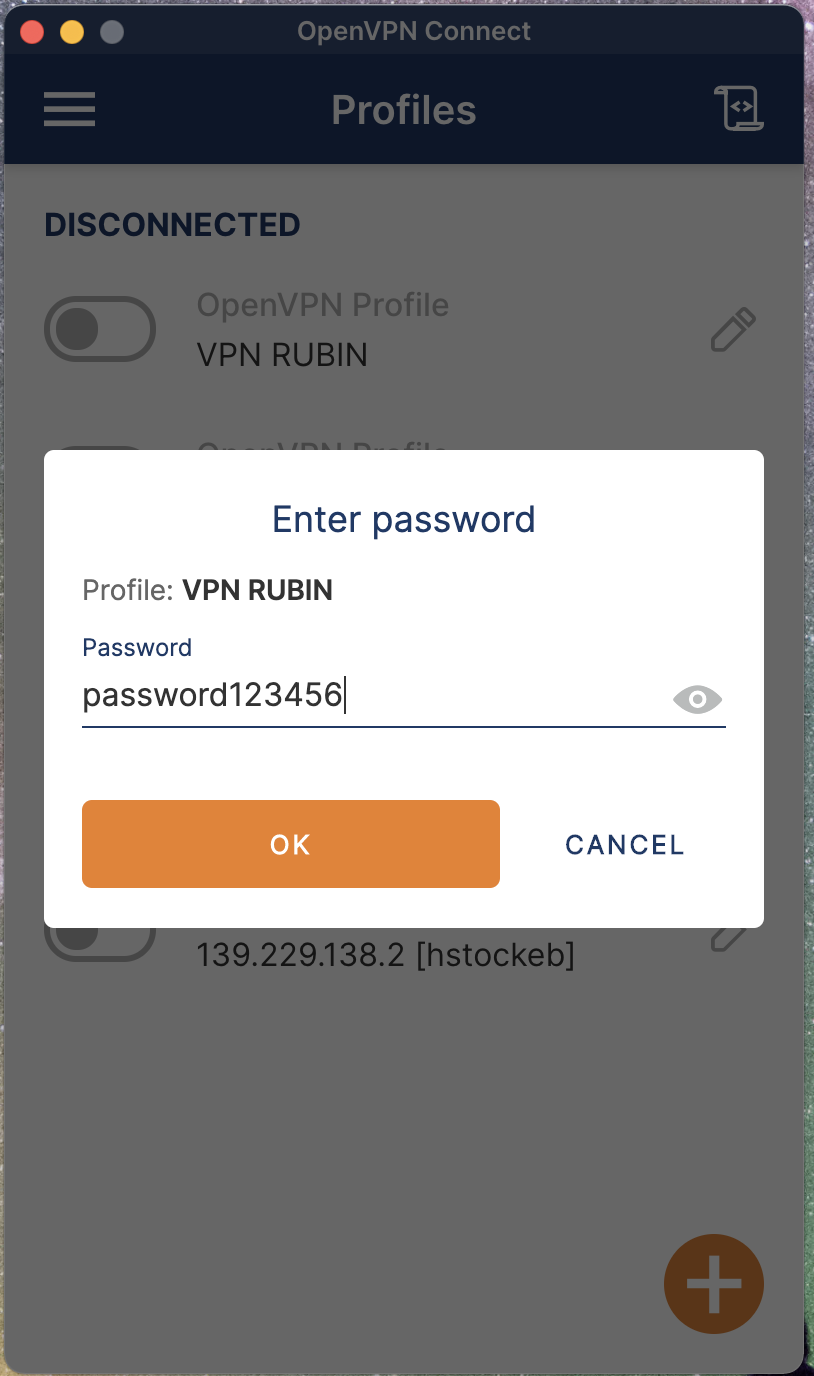
\includegraphics[width=50mm]{images/vpn_password.png}
    \caption{Password field on OpenVPN Connect client}
    \label{fig:label}
\end{figure}

The feature of a new field or a box requesting the OTP code is only available on the paid version of OpenVPN Acces Server.
So this can be a litle confusing to users, due to the way to write the password and code on the same field.




\newpage
\section{DUO Authentication}

\begin{figure}[!h]
  \centering
  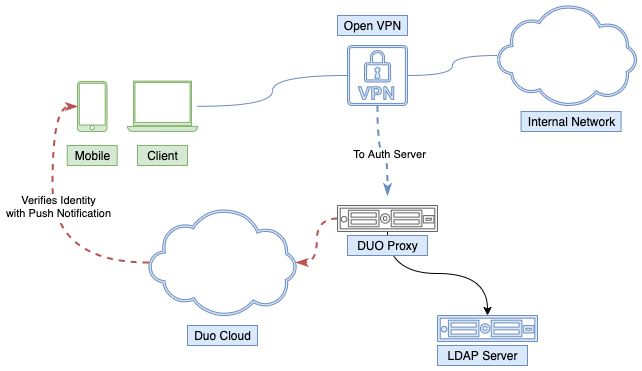
\includegraphics[width=160mm]{images/DUO-Proxy.drawio.png}
  \caption{OpenVPN + DUO Proxy}
  \label{fig:label}
\end{figure}

\href{https://duo.com/}{Duo Security} is a security platform that provides push notifications to autorize or deny a user login, on our case a VPN connection.

Users can be syncronized to the Duo Dashboard, to automatically enroll users sending a Welcome Email, leting the user install and sync the account with the app on his smarthphone.

On this case a service called "Proxy" is need to be install on la machine inside the local network. On the OpenVPN configuration a change is needed on the authentication servers, now it need to be pointed to the proxy, so besides sending a ldap request to the local ldap server, it will request authization to the user via the app recently installed on this smartphone.

Temporary Text



\subsection{Test}


\newpage
\section{Final Toughs}



\section{Abstract}
The Following documents details how to enable and configure two-factor authentication (2FA) for Rubin Observatory OpenVPN users

\appendix
% Include all the relevant bib files.
% https://lsst-texmf.lsst.io/lsstdoc.html#bibliographies
\section{References} \label{sec:bib}
\renewcommand{\refname}{} % Suppress default Bibliography section
\bibliography{local,lsst,lsst-dm,refs_ads,refs,books}

% Make sure lsst-texmf/bin/generateAcronyms.py is in your path
\section{Acronyms} \label{sec:acronyms}
\addtocounter{table}{-1}
\begin{longtable}{p{0.145\textwidth}p{0.8\textwidth}}\hline
\textbf{Acronym} & \textbf{Description}  \\\hline

PMO & Project Management Office \\\hline
VPN & virtual private network \\\hline
\end{longtable}

% If you want glossary uncomment below -- comment out the two lines above
%\printglossaries





\end{document}
